\section{Implementation}
\label{sec:impl}

On end hosts, \sys is a reliable transport built upon RDMA/RoCEv2 unreliable datagram or UDP.
This section implements packet processing in three types of network switches with different programming capabilities.

\begin{figure*}[t]
\centering
\subfloat[Data-plane programmable switches.\label{fig:p4}]
{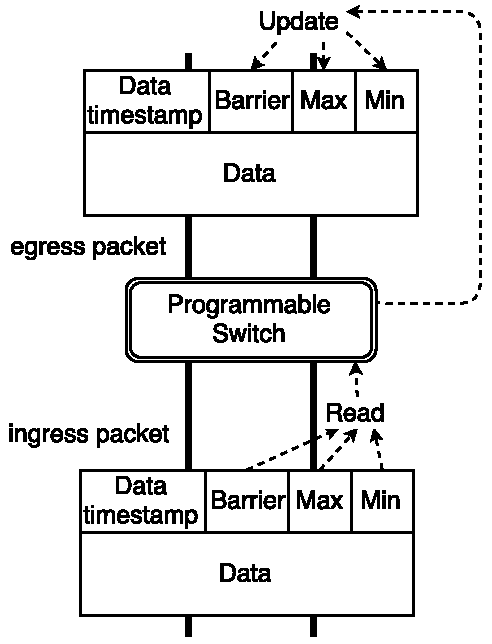
\includegraphics[width=.3\textwidth]{images/p4_implementation.pdf}}
\hspace{0.04\textwidth}
\subfloat[CPU on commodity switches.\label{fig:commodity}]
{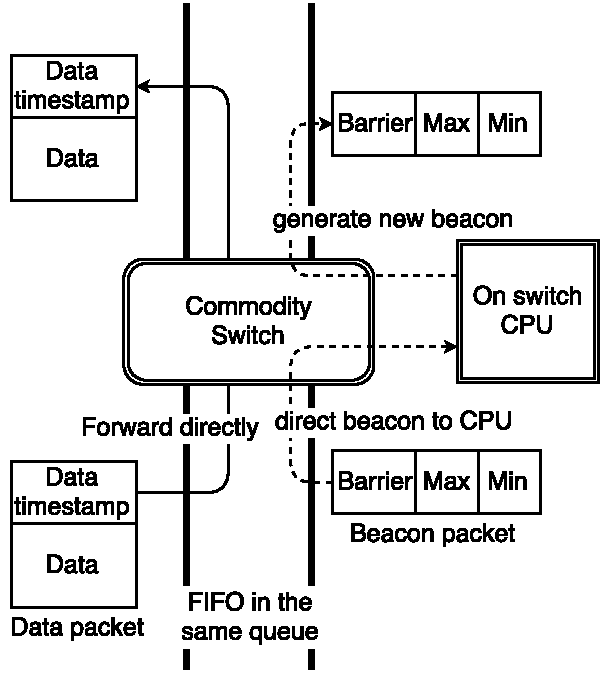
\includegraphics[width=.3\textwidth]{images/commodity_implementation.pdf}}
\hspace{0.04\textwidth}
\subfloat[End hosts only.\label{fig:end-host}]
{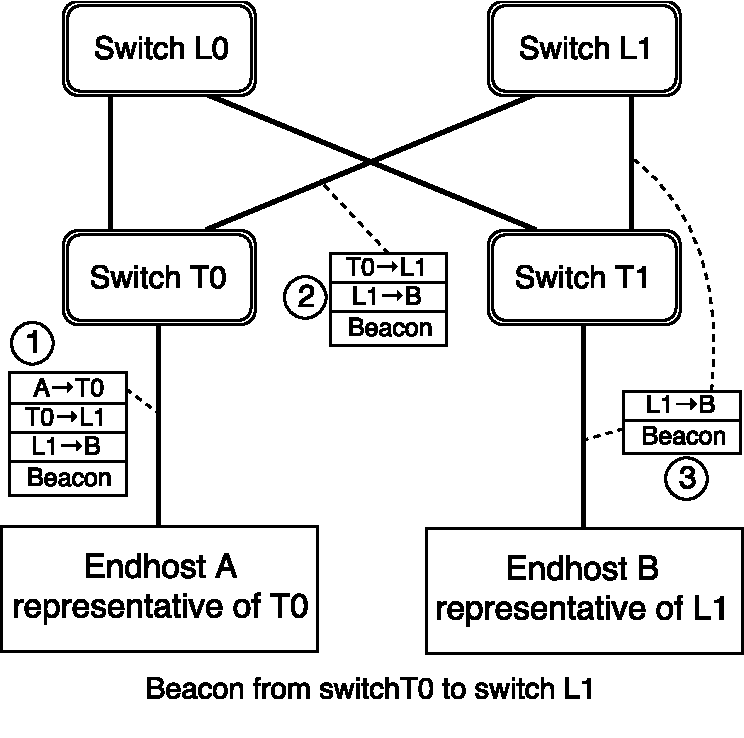
\includegraphics[width=.3\textwidth]{images/endhostonly_implementation.pdf}}
\caption{\sys dataflow in networks with different programming capabilities.}
\label{fig:impl}
\vspace{-1em}
\end{figure*}

\subsection{Data-plane Programmable Switches}
\label{sec:p4}

A data-plane programmable switch is able to maintain a handful of states $\mathcal{S}$ and process each packet $P$ through the state machine $P', \mathcal{S}' = f(P, \mathcal{S})$.
To implement \sys, there needs to be 8 state registers per ingress port and 5 state registers per egress port.
Each data packet carry three timestamps: a data timestamp, an unreliable barrier and an ACK barrier, as well as a loss encountered binary flag (Algorithm~\ref{alg:loss-detection}).
Each timestamp is a 6-byte integer, indicating the number of nanoseconds passed. Since the timestamps wrap around in 7.8 hours, we use PAWS~\cite{jacobson1992tcp} to compare timestamps: If $s$ and $t$ are timestamp values, $s < t$ iff $0 < t - s < 2^{47}$, computed in 48-bit unsigned arithmetic.
As shown in Figure~\ref{fig:p4}, the beacon packets carry not only the same set of timestamps and flag as data packets, but also information for minimax clock synchronization (Algorithm~\ref{alg:minimax}).

\subsection{CPU on Commodity Switches}
\label{sec:commodity}

Data-plane programmable switches are currently not widely available in data centers. Although commodity switches cannot process packets in data plane, they have a CPU to process control-plane packets, analogous to directly connecting a server to a port of the switch. Compared to server CPUs and NICs, the switch CPUs are typically less powerful (\textit{e.g.}, 4 cores at 1~GHz) and has lower bandwidth (\textit{e.g.}, 1 Gbps).

Because the CPU is not capable of processing every data packets, we again rely on the principle of separating control from data. The control is consisted of beacon packets carrying timestamp information. As shown in Figure~\ref{fig:commodity}, regular data packets is forwarded by the switch as if there were no \sys service, and stored in reorder buffer on end-host receivers. The end-host senders send beacons periodically, regardless of whether the link is idle or busy. The beacon packets are sent to the switch CPU for processing. Because data and beacon packets are FIFO in the switch queues and on the network links, the barrier property is preserved. On end-host receivers, the buffered data packets are delivered to the application according to barriers in beacon packets.

Compared with the previous approach, this approach slacks the barriers in two aspects. First, the barriers are updated periodically by beacons only instead of by every packet. Second, the processing delay of beacon packets in switch CPU is longer than the processing delay of data packets by switching chip.
The worst-case reordering delay added by the slack, is (beacon interval + processing delay) $\times$ number of hops.
In practice, Algorithm~\ref{alg:beacon} can synchronize beacon intervals on different hops, so the additional reordering delay is beacon interval + (processing delay $\times$ number of hops).

\subsection{End Hosts Only}
\label{sec:end-host}

In case the switch vendor does not allow programming in switch CPUs, we can still implement \sys by offloading the beacon processing to end hosts. The challenge is to maintain the FIFO property. Beacons with barrier timestamps on a network link $L$ must pass through $L$. To this end, we designate an \textit{end-host representative} for each network switch. The location of the representative is arbitrary and does not need to be unique, but it is more efficient to be close to the switch.

As shown in Figure~\ref{fig:end-host}, for two directly-connected switches $S_1, S_2$ and their representatives $H_1, H_2$, beacon packets from $H_1$ to $H_2$ need to go through the link $S_1 \rightarrow S_2$. A beacon packet $H_1 \rightarrow H_2$ is sent with three layers of IP headers: $H_1 \rightarrow S_1$, $S_1 \rightarrow S_2$ and $S_2 \rightarrow H_2$. We install tunnel termination rules in each network switch to decapsulate one layer of IP header, so the beacon packet will traverse through $H_1 \rightarrow S_1 \rightarrow S_2 \rightarrow H_2$.

The beacon processing delay overhead of offloading a switch to an end-host representative is the RTT from the end host to the switch. %Compared to Sec.~\ref{sec:commodity}, the additional reordering delay is host-to-switch RTT $\times$ number of hops.
